\documentclass[a4paper,12pt]{report}
\usepackage{styles/fbe_tez}
% V2: center the existing 155 mm text block on the physical page.
% Override the thesis binding margin without modifying the supplied style.
\setlength{\oddsidemargin}{\dimexpr(\paperwidth-\textwidth)/2-1in-\hoffset\relax}
\setlength{\evensidemargin}{\oddsidemargin}
\usepackage{iftex}
\ifPDFTeX
  \usepackage[T1]{fontenc}
  \usepackage[utf8]{inputenc}
\else
  \usepackage{fontspec}
  \setmainfont{lmroman12-regular.otf}[
    BoldFont=lmroman12-bold.otf,
    ItalicFont=lmroman12-italic.otf,
    BoldItalicFont=lmroman10-bolditalic.otf]
\fi
\usepackage{amsmath,amssymb}
\usepackage[bottom]{footmisc}
\usepackage{cite,url,graphicx,longtable,array,booktabs,float}
\usepackage{tikz}
\usetikzlibrary{arrows.meta,positioning,fit,shapes.geometric}
\usepackage[hidelinks,breaklinks]{hyperref}
\renewcommand{\labelenumi}{(\roman{enumi})}
\newcolumntype{L}[1]{>{\raggedright\arraybackslash}p{#1}}
\newcommand{\tuik}{T\"U\.{I}K}
\newcommand{\code}[1]{\texttt{\small #1}}
\newenvironment{singlespace}{\begingroup\renewcommand{\baselinestretch}{1}\selectfont}{\par\endgroup}
\newcommand{\studentone}{Ahmet Baha Bayrakçıoğlu}
\newcommand{\studenttwo}{Ökkeş Berkay Acer}
\newcommand{\projectadvisor}{Can Özturan}
\emergencystretch=2em
\hypersetup{pdftitle={MCP Server for TÜİK Data - Midterm Report},pdfauthor={Ahmet Baha Bayrakçıoğlu and Ökkeş Berkay Acer}}
\tikzset{box/.style={draw,rounded corners=2pt,align=center,minimum height=9mm,text width=34mm,font=\small},arr/.style={-{Stealth[length=2mm]},thick},entity/.style={draw,align=left,text width=56mm,font=\small,inner sep=7pt}}

\begin{document}
\title{CMPE 492 \\ MCP Server for \tuik{} Data \\[0.5em] Midterm Report}
\author{\studentone{} \textbar{} 2022400051 \\ \studenttwo{} \textbar{} 2022400066 \\ \\ Advisor: \\ \projectadvisor}
\date{November 2026}
\hypersetup{pageanchor=false}
\maketitle
\pagenumbering{roman}
\hypersetup{pageanchor=true}
\tableofcontents

\chapter{INTRODUCTION}
\pagenumbering{arabic}
Official statistics support research, journalism and public discussion, but finding a suitable source and retrieving its actual observations are different tasks. A user looking for unemployment statistics may encounter a bulletin, a methodology page, an Excel attachment and a downloadable dataflow. These resources have different structures and access paths. Their titles alone do not establish whether they contain the requested period, population or geographical breakdown.

This project develops \emph{MCP Server for \tuik{} Data}, a Python server that connects Model Context Protocol (MCP) clients to publicly accessible resources of the Turkish Statistical Institute. The server provides structured tools for discovery, metadata inspection, bounded table retrieval, PDF reading and chart generation. The language model remains in the client: the server retrieves and processes source material rather than generating statistical answers itself. MCP supplies the interface through which the client discovers and invokes these operations \cite{mcp-tools}.

The main engineering problem is to make heterogeneous official resources usable without losing their meaning or provenance. Accordingly, the implementation preserves source labels, units, notes, retrieval times and missing-value markers. An optional Turkish lexical index and conditional hybrid ranking improve discovery while the official source remains authoritative for resource resolution and data retrieval.

This midterm report covers the implementation and evidence available on 11 November 2026. The report includes the GitHub development revision \code{759c26e} (merged PR 77), dated 5 November, in addition to the local implementation snapshot \code{e3e991b}. Version 0.3.0 was published on 5 November, and optional hybrid search was subsequently merged into the development branch. Nine MCP tools, recorded acceptance checks and frozen lexical/hybrid relevance experiments are available. Further ranking improvements and final deliverables remain work in progress \cite{project,acceptance,hybrid,release-record}.

\section{Broad Impact}
The intended benefit is easier, traceable access to official statistics from a conversational or analytical workflow. Students and researchers can discover sources, inspect actual column names and request a bounded subset without writing a separate scraper for each file format. Journalists and other users can follow the same source links when checking a result. These are intended benefits; a reduction in user effort has not yet been quantified through a user study.

The project also demonstrates a reusable pattern for connecting language-model clients to public information services: narrow tools, explicit source identities, bounded execution and visible failure states. Caching and paced downloads reduce repeated requests to the upstream service. The software runs locally and does not require a model service or API key inside the server, although the chosen MCP client may have its own requirements.

\section{Ethical Considerations}
Access to a credible publisher does not make every interpretation correct. A national unemployment rate cannot substitute for a provincial or demographic rate, and a current bulletin need not contain the historical period requested by a user. The server therefore exposes source context and avoids inventing dimensions or converting missing markers into zero. Chart generation preserves gaps and reports the rows and series used.

Only publicly accessible operations are implemented. The project does not obtain credentials, bypass authentication or retrieve restricted microdata. Upstream 401/403 responses remain errors. Public availability is not treated as permission to redistribute every underlying publication without checking applicable conditions. Attribution is retained, and the server is not presented as an official \tuik{} product.

Retrieved text is untrusted data. Instructions embedded in a source document must not become executable instructions for the server or client. The network layer restricts fetched URLs to verified HTTPS hosts; parsers do not execute spreadsheet macros or formulas. Download, parsing and response budgets limit ordinary resource consumption, although thread-based parsing is not a hard process-memory sandbox.

The lexical relevance experiment uses one AI assessor followed by a dependent source review. The later hybrid experiment retains those labels and adds a second AI model's assessment and review of new pairs; neither provides independent human validation. The team additionally reports limited manual trials of the system, without a retained quantitative human relevance study. These trials are treated as qualitative checks and are not used to relabel the recorded AI experiment as independent human validation.

\chapter{PROJECT DEFINITION AND PLANNING}
\section{Project Definition}
The objective is a locally runnable MCP server for discovering and reading public \tuik{} statistical resources through a consistent interface. Its implemented scope comprises portal and dataset search; bulletin and file metadata; statistical themes and classification search; CSV, XLS and XLSX rows; PDF page text and best-effort tables; bounded queries; and optional line or bar charts.

An optional OpenSearch service supplies Turkish-aware lexical discovery over derived metadata and selected file content. With the semantic dependency, cached embedding model and compatible vector index present, mixed-kind metadata search additionally combines lexical and semantic rankings. It is not a replacement statistical database. Reads resolve stable resource identities against official sources and verify downloadable files. If the index is absent or unavailable, the server reports a fallback to literal dataset matching or live portal search with the relevant limitations.

The present scope excludes authenticated SDMX retrieval, unrestricted SQL, OCR, execution of user code and a standalone graphical frontend. Optional hybrid metadata retrieval is implemented on the development branch; dataset-only and file-content retrieval remain lexical. Full historical file coverage and production hosting are also outside the completed scope.

\section{Project Planning}
Development has proceeded in increments: first establish public source access, then make file retrieval reliable, and finally improve discovery and collect evaluation evidence. Table~\ref{tab:plan} separates the observed work from the proposed remaining schedule. Dates after the reporting cutoff are proposed estimates rather than confirmed team commitments. The technical follow-ups match open GitHub issues 78--80 \cite{remaining-issues}.

\subsection{Project Time and Resource Estimation}
\begin{table}[H]
\caption{Observed milestones and proposed remaining work.}
\label{tab:plan}
\centering\renewcommand{\baselinestretch}{1}\small\renewcommand{\arraystretch}{1.15}
\begin{tabular}{L{26mm} L{94mm} L{22mm}}
\toprule Period & Work package & Status \\
\midrule
13--17 Oct. & Public-source investigation, initial MCP operations and dataset discovery. & Completed \\
18--22 Oct. & Download pacing, reusable file IDs, Excel/PDF readers, limits and caching. & Completed \\
26--29 Oct. & Turkish analysis, metadata crawler/indexer, inspection and bounded table queries. & Completed \\
2--5 Nov. & Indexed discovery, content checks, charts, lexical/hybrid experiments and published 0.3.0. & Completed \\
11--17 Nov. & Midterm review, advisor feedback and report revision. & Planned \\
18 Nov.--6 Dec. & Group repeated bulletin series (issue 78), recover hybrid abbreviation queries (79), and evaluate dataset-filtered hybrid ranking (80). & Planned \\
7--14 Dec. & Task-level validation, clean installation checks and stabilization of subsequent development changes. & Planned \\
15--21 Dec. & Final report, poster, short video and presentation preparation, subject to confirmed course dates. & Planned \\
\bottomrule
\end{tabular}
\end{table}

The main resources are two student developers, ordinary development computers, Python 3.12 or newer, Git/GitHub and a local container runtime for index experiments. The development OpenSearch container uses a 512 MiB Java heap; this is a configuration value, not measured total memory consumption. Parsing and search libraries are open source. No dedicated GPU or paid inference service is required by the implemented server. A client using an external language model may incur separate costs.

Remaining effort is estimated as approximately four weeks of validation and refinement followed by one week of final deliverable preparation. Actual person-hours have not been logged, so retrospective effort totals are not claimed. Ranking changes should be accepted only after the existing discovery-to-reading workflow remains reproducible.

\subsection{Success Criteria}
The midterm criteria are: a client can discover the tool schemas; a search result can be followed to official metadata and supported rows or document text; every response retains provenance; invalid requests and unavailable sources produce explicit errors; and optional search failure does not prevent supported live reads. Repeated reads must obey bounded caches and queries must not silently change their source snapshot during pagination.

For discovery quality, a frozen query set must support reproducible comparison of Turkish lexical configurations. The present experiment satisfies this engineering comparison criterion with disclosed AI judgments. Broader success at the final stage requires clearer evidence of end-to-end user tasks, coverage of known failure cases and a reviewable installation and demonstration package. No universal accuracy or latency threshold is retroactively asserted.

\subsection{Risk Analysis}
\begin{table}[H]
\caption{Principal project risks and current responses.}
\label{tab:risks}
\centering\renewcommand{\baselinestretch}{1}\small\renewcommand{\arraystretch}{1.15}
\begin{tabular}{L{34mm} L{46mm} L{62mm}}
\toprule Risk & Consequence & Mitigation / remaining limitation \\
\midrule
Internal portal API changes & Search or parsing contracts break. & Isolated adapters, recorded fixtures and optional live contract monitoring; no upstream stability guarantee. \\
Rate limits / rotating links & Failed or stale downloads. & Six-second file spacing, bounded retries and fresh identity resolution. \\
Unexpected file layouts & Misaligned columns or lost context. & Real-file tests, preserved notes, raw-layout warnings and explicit limits. \\
Stale or incomplete index & Missing or misleading discovery. & Retrieval/index timestamps, validated full rebuilds, atomic alias switch and explicit fallback. \\
Turkish lexical ambiguity & Relevant sources remain unseen. & Separate Turkish/ASCII fields, reviewed synonyms, failure analysis and bounded fuzziness. \\
Evaluation bias & Overstated retrieval quality. & Frozen evidence and disclosed dependent AI review; independent human validation remains open. \\
Late scope expansion & Incomplete final deliverables. & Prioritize core task checks and documented ranking follow-ups before expanding scope. \\
\bottomrule
\end{tabular}
\end{table}

\subsection{Team Work (if applicable)}
The team consists of \studentone{} and \studenttwo{}, with \projectadvisor{} as the project advisor. Work is organized through issues, topic branches, pull requests and a shared changelog. CI covers Python checks, repository automation, container building and optional search integration. Topic changes are reviewed before integration, and release preparation is distinguished from publication. This report presents the joint system; a person-by-person work-hour or feature allocation is not inferred from commit counts.

\chapter{RELATED WORK}
Public statistical portals already provide authoritative publications and exports. The \tuik{} portal is both the upstream service and the natural manual baseline for this project \cite{tuik-portal}. The server adds a programmatic workflow around its heterogeneous resources; it does not produce an alternative statistical series. The recorded source investigation found public frontend endpoints and a separate authenticated SDMX route. The latter was excluded from the implemented anonymous-access workflow \cite{source-investigation}.

SDMX addresses the exchange of statistical data and metadata through shared structures and standards \cite{sdmx}. MCP serves a different integration layer: it exposes named operations and schemas to a client application \cite{mcp-tools}. The project combines statistical-source adapters with MCP tools, using the official Python SDK's FastMCP implementation \cite{mcp-sdk}. It neither implements the SDMX standard nor assumes every \tuik{} resource is available through one observation endpoint.

For Turkish retrieval, OpenSearch provides a built-in language analyzer and configurable token filters. Its synonym graph filter supports multiword alternatives \cite{os-turkish,os-synonyms}. These facilities make it possible to compare a built-in baseline against a custom multi-field chain while retaining inspectable token behavior. The project additionally separates original Turkish text from ASCII-folded title matching, because folding and stemming in the wrong order can lose useful distinctions. This design is supported by retained project probes, not a claim of complete Turkish morphological analysis.

Lewis et al. combine external retrieval with generation for knowledge-intensive language tasks \cite{rag}. This server supplies source material to a client without training a generator; its optional semantic path uses a pretrained multilingual embedding model. For the retrieval experiments, graded relevance and discounted cumulative gain distinguish direct answers from contextual matches \cite{ndcg}. Multiple metrics capture both ranking and coverage.

\chapter{METHODOLOGY}
\section{Source-grounded Development}
Development starts from observed official responses. Portal JavaScript and public pages were inspected to identify search, bulletin, category, export and classification access paths. The adapters validate these responses rather than constructing undocumented statistical dimensions or opaque download parameters. Small retained responses and a 12-file official fixture corpus support repeatable tests without repeated network traffic \cite{source-investigation,project}.

The workflow is discovery, resolution, inspection and retrieval. Search returns an identity and provenance; resolution identifies the available source and downloads; inspection reveals exact column keys and observed values; retrieval applies a bounded operation to the selected file. The distinction between an advertised export and a verified download is retained throughout. A bulletin exposing several dataflows returns choices rather than silently selecting one.

\section{Preserving Statistical Meaning}
CSV and spreadsheet observations remain strings in the public row representation. Parsers preserve printed precision, multi-row labels, units, notes and placeholder symbols. XLS/XLSX heuristics reconstruct recognized table layouts; unfamiliar layouts remain available as raw grids with warnings. PDF extraction deduplicates overlapping glyphs and returns physical page numbers with character-offset continuation. Scanned pages are reported as lacking a text layer.

Typed table predicates are local operations on a downloaded snapshot. Numeric and date interpretation is conservative: ambiguous separators require explicit guidance rather than a guessed conversion. Stable sorting uses source position to break ties. A continuation cursor binds to the retained result and query; expiration or eviction requires a new query instead of silently downloading a newer table. Charts consume the same bounded data path and show gaps rather than inventing zero observations.

\section{Turkish Lexical Retrieval}
The optional index stores normalized metadata with source identities. The original-text chain normalizes apostrophes, applies Turkish lowercase and stems Turkish tokens. A separate ASCII path applies Turkish lowercase before ASCII folding and avoids stemming the folded title. Search-time graph synonyms cover abbreviations and selected broader expressions. Exact keyword fields support resource type, theme, date and advertised-downloadability filters.

Retrieval combines weighted title, description, body and theme evidence with a weaker, bounded ASCII fuzzy clause. The design does not guarantee recovery of every suffix or typo: retained probes fail for examples such as \code{issizligin}, and a misspelled synonym trigger need not activate the intended expansion. File-content discovery is opt-in by resource kind and returns a page or worksheet locator. It indexes PDF passages and workbook descriptive material, not all statistical cell values.

\section{Implemented Hybrid Retrieval}
The development branch adds \code{intfloat/multilingual-e5-small}, run through optional fastembed/ONNX, to embed metadata documents and queries. The indexer writes vectors for dataflows, bulletins and metadata records. The runtime uses locally cached model files and combines lexical retrieval with filtered nearest-neighbor retrieval using equal-weight reciprocal rank fusion in OpenSearch \cite{hybrid}.

Hybrid ranking requires compatible vectors and model files. Dataset-only requests, workbook/PDF content searches and deeper pages remain lexical; unavailable semantic prerequisites or a failed hybrid request trigger the documented lexical path. Responses expose \code{ranking} so clients can distinguish the executed path. The base installation remains usable without a model dependency. No generator is trained by this extension.

\section{Evaluation Protocol}
The retrieval experiment freezes 48 queries in eight categories, six per category: exact titles, abbreviations, synonyms, inflections, ASCII typing, typos, multiple concepts and regional needs. Three OpenSearch variants use the same 3,424-document snapshot. Portal search and literal dataset matching are also recorded, with their different corpus boundaries explicitly identified \cite{evaluation}.

The lexical pool contains 1,390 query--document pairs over 608 documents, graded 0 (unrelated), 1 (contextual) or 2 (directly relevant). One Codex assessment and dependent source review produced 55 revisions. The hybrid experiment retains those grades and adds 299 pairs, reaching 1,689 pairs over 748 documents. Claude graded and reviewed the additions, with nine revisions, while also implementing the hybrid systems. Neither stage supplies independent human judgments or inter-rater agreement \cite{hybrid}.

For a query with grades $g_i$, the implementation computes
\begin{equation}
 \mathrm{DCG@10}=\sum_{i=1}^{10}\frac{2^{g_i}-1}{\log_2(i+1)},
 \qquad \mathrm{nDCG@10}=\frac{\mathrm{DCG@10}}{\mathrm{IDCG@10}}.
\end{equation}
MRR@10 averages the reciprocal rank of the first grade-positive result in the top ten. Pooled Recall@10 measures retrieved grade-positive documents against known relevant pooled documents eligible for that system. It is not exhaustive recall over every relevant official resource. Query-level scores are macro-averaged; zero-known-relevant queries receive zero. The results chapter interprets the measured differences within these boundaries.

\chapter{REQUIREMENTS SPECIFICATION}
\section{Actors and Use Cases}
The primary actor is a user operating an MCP-compatible client. The client invokes tools on the user's behalf. An index maintainer is a separate operational actor who runs explicit crawl/build commands; normal MCP reading does not write the index. Figure~\ref{fig:usecase} summarizes these responsibilities.

\begin{figure}[H]
\centering
\begingroup\renewcommand{\baselinestretch}{1}\selectfont
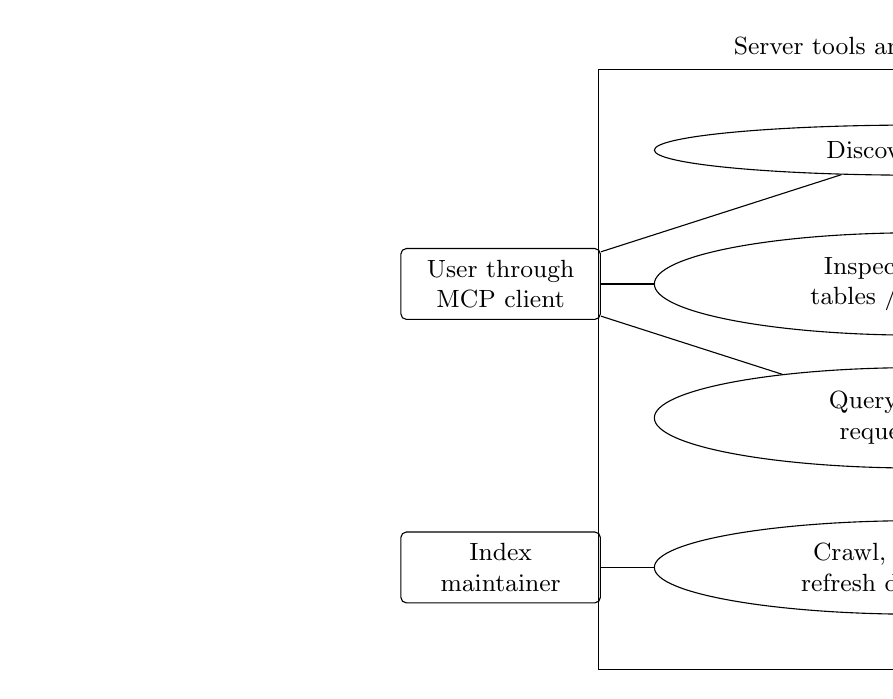
\begin{tikzpicture}[x=1cm,y=1cm]
\node[box,text width=23mm] (user) at (-1,0) {User through\\MCP client};
\node[draw,ellipse,align=center,font=\small,text width=45mm] (s) at (4.3,1.7) {Discover sources};
\node[draw,ellipse,align=center,font=\small,text width=45mm] (r) at (4.3,0) {Inspect and read\\tables / documents};
\node[draw,ellipse,align=center,font=\small,text width=45mm] (c) at (4.3,-1.7) {Query rows and\\request charts};
\node[box,text width=23mm] (maint) at (-1,-3.6) {Index\\maintainer};
\node[draw,ellipse,align=center,font=\small,text width=45mm] (idx) at (4.3,-3.6) {Crawl, rebuild and\\refresh derived index};
\draw (user)--(s);\draw (user)--(r);\draw (user)--(c);\draw (maint)--(idx);
\node[draw,fit=(s)(r)(c)(idx),inner sep=7mm,label={[font=\small]above:Server tools and operational CLI}] {};
\end{tikzpicture}
\endgroup
\caption{Use-case overview. Reading and index maintenance have separate entry points.}
\label{fig:usecase}
\end{figure}

\clearpage
\section{Functional Requirements}
\setlength{\LTcapwidth}{\textwidth}
\begin{longtable}{L{13mm} L{88mm} L{40mm}}
\caption{Functional requirements and midterm verification paths.}\label{tab:req}\\
\toprule ID & Requirement & Verification \\
\midrule\endfirsthead
\toprule ID & Requirement & Verification \\
\midrule\endhead
FR1 & Discover public resources and reusable export-dataset IDs, with explicit backend and filter limitations. & Search contracts; indexed/live smoke. \\
FR2 & Resolve metadata, source URLs, downloads and related dataflows. & Identity and bulletin tests. \\
FR3 & Return bounded CSV/XLS/XLSX rows with exact filters and worksheet selection. & Parser fixtures; live row checks. \\
FR4 & Inspect exact columns, observed values and conservative type hints before filtering. & Profile and snapshot tests. \\
FR5 & Support projection, typed predicates, stable sorting and snapshot-bound continuation. & Query boundary and cursor tests. \\
FR6 & Read bounded PDF text with lossless continuation and optional best-effort page tables. & PDF fixtures and continuation tests. \\
FR7 & Generate optional PNG line/bar charts with source context and gaps preserved. & Offline chart tests. \\
FR8 & List major themes and search public classification editions. & Adapter tests and live smoke. \\
FR9 & Optionally index metadata and selected file content, returning usable page/sheet locators. & Crawler/indexer and real-cluster tests. \\
\bottomrule
\end{longtable}

\section{Non-functional Requirements}
Provenance is mandatory: responses include \code{source\_url}, \code{retrieved\_at} and \code{publisher}, with individual-record provenance for collections. Retrieval and indexing times have different meanings and must not be conflated. An advertised file must not be marked verified before it has been fetched and checked.

Reliability requires timeouts, bounded retries, shared pacing, explicit error codes and compatibility with unconfigured search. Resource use is controlled by input limits, byte-bounded caches, serialized parsing and output budgets. The base installation must operate without optional visualization, OpenSearch or semantic-model dependencies. Maintainability requires isolated source adapters, network-free parsers, a backend interface and reproducible fixtures. The midterm evidence tests these properties; it does not establish a production service-level agreement.

\chapter{DESIGN}
\section{Information Structure}
The system has no canonical relational database. Official resources are represented by stable identities, while parsed snapshots and index records are derived views. Figure~\ref{fig:entities} shows their conceptual relationships; it is not a physical SQL schema.

\begin{figure}[H]
\centering
\begingroup\renewcommand{\baselinestretch}{1}\selectfont
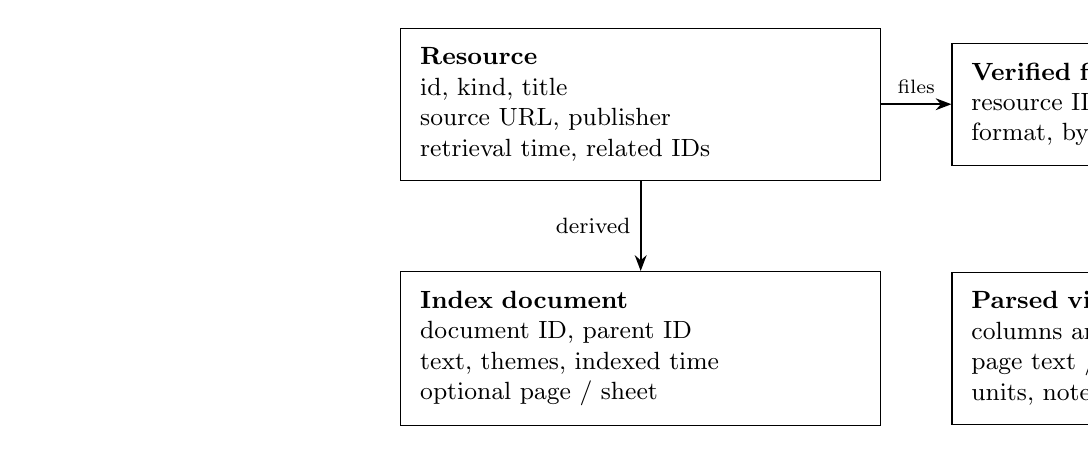
\begin{tikzpicture}
\node[entity] (res) at (0,0) {\textbf{Resource}\\id, kind, title\\source URL, publisher\\retrieval time, related IDs};
\node[entity] (file) at (7,0) {\textbf{Verified file snapshot}\\resource ID, SHA-256\\format, bytes, retrieval time};
\node[entity] (idx) at (0,-3.1) {\textbf{Index document}\\document ID, parent ID\\text, themes, indexed time\\optional page / sheet};
\node[entity] (parsed) at (7,-3.1) {\textbf{Parsed view}\\columns and string rows, or\\page text / tables\\units, notes, warnings};
\draw[arr] (res)--node[above,font=\scriptsize]{files}(file);
\draw[arr] (res)--node[left,font=\footnotesize]{derived}(idx);
\draw[arr] (file)--node[right,font=\footnotesize]{1..* views}(parsed);
\end{tikzpicture}
\endgroup
\caption{Conceptual information structure and derived representations.}
\label{fig:entities}
\end{figure}

Catalog dataflows use \code{flow:} identities; bulletins use \code{press:} identities. File identities use a title-derived key, with disambiguation where needed, because opaque download links rotate. They identify the current source file with that identity, not an immutable historical revision. A file's content hash identifies a particular retained snapshot. Some classification and generic resource handles remain bounded session handles and must be searched again after expiry.

An index document stores type, text, confirmed categories, advertised formats, related IDs and source/index timestamps. Content records additionally reference a parent file and physical page or worksheet. The strict schema rejects unknown fields. Query continuation state separately binds a normalized query to a retained snapshot and expires after a configured interval.

\section{Information Flow}
Figure~\ref{fig:flow} illustrates a successful table-reading path. Search is a discovery step; verification occurs later. A cache hit reuses its original timestamp, and cursor continuation remains on the same retained snapshot.

\begin{figure}[H]
\centering
\begingroup\renewcommand{\baselinestretch}{1}\selectfont
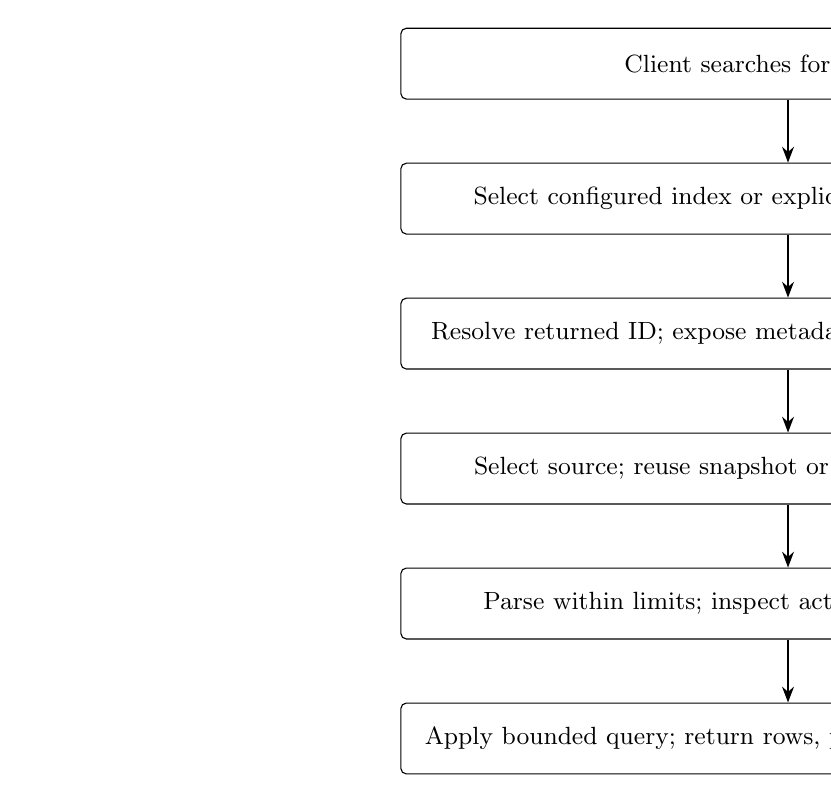
\begin{tikzpicture}[node distance=8mm]
\node[box,text width=96mm] (a) {Client searches for a resource};
\node[box,text width=96mm,below=of a] (b) {Select configured index or explicit portal/literal fallback};
\node[box,text width=96mm,below=of b] (c) {Resolve returned ID; expose metadata and file/dataflow choices};
\node[box,text width=96mm,below=of c] (d) {Select source; reuse snapshot or fetch paced, verified file};
\node[box,text width=96mm,below=of d] (e) {Parse within limits; inspect actual columns and values};
\node[box,text width=96mm,below=of e] (f) {Apply bounded query; return rows, provenance and continuation};
\draw[arr](a)--(b);\draw[arr](b)--(c);\draw[arr](c)--(d);\draw[arr](d)--(e);\draw[arr](e)--(f);
\end{tikzpicture}
\endgroup
\caption{Discovery-to-query activity flow. Failures at each stage return explicit status or error information.}
\label{fig:flow}
\end{figure}

PDF reading follows the same resolution/download path, then extracts the requested physical page. If the character bound cuts a page, the next request continues at an offset on that page before moving forward. File-content search can enter this path directly using a returned file identity and page or sheet.

Index maintenance is a separate flow: enumerate official metadata, validate unique IDs and expected totals, normalize records, prepare a new physical index, verify its document count and atomically switch the alias. Failed crawls or writes do not advance the stored checkpoint. Incremental builds upsert changed records and report stale IDs; full rebuilds establish a clean snapshot.

\section{System Design}
\begin{figure}[H]
\centering
\begingroup\renewcommand{\baselinestretch}{1}\selectfont
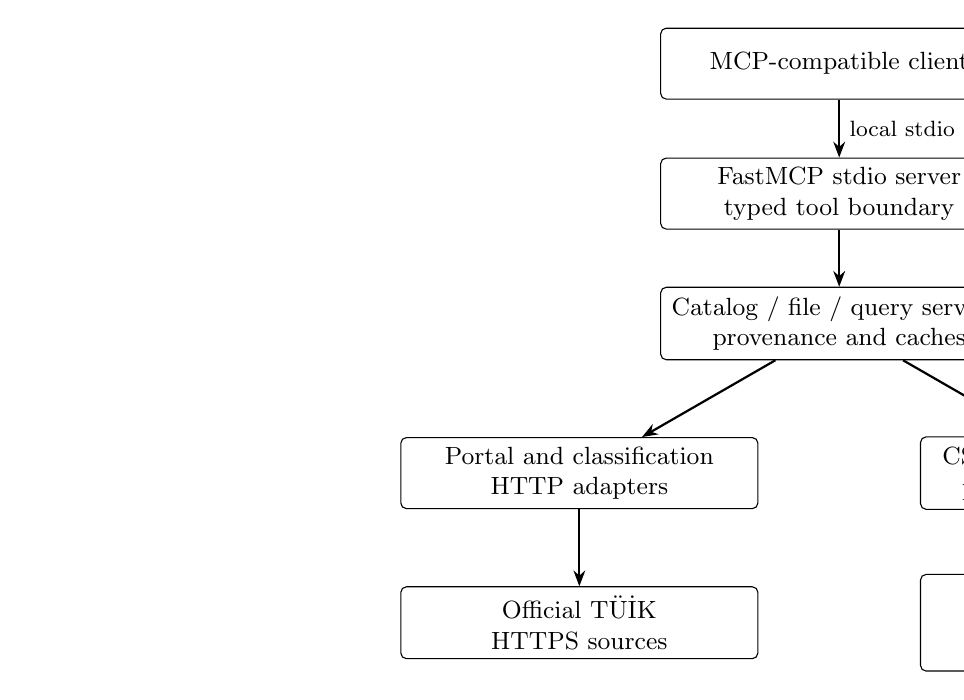
\begin{tikzpicture}
\node[box,text width=43mm] (client) at (0,0) {MCP-compatible client};
\node[box,text width=43mm] (server) at (0,-1.65) {FastMCP stdio server\\typed tool boundary};
\node[box,text width=43mm] (svc) at (0,-3.3) {Catalog / file / query services\\provenance and caches};
\node[box,text width=43mm] (adp) at (-3.3,-5.2) {Portal and classification\\HTTP adapters};
\node[box,text width=43mm] (parse) at (3.3,-5.2) {CSV / Excel / PDF parsers\\profile, query and charts};
\node[box,text width=43mm] (official) at (-3.3,-7.1) {Official \tuik{} HTTPS sources};
\node[box,text width=43mm] (index) at (3.3,-7.1) {Optional OpenSearch\\derived index\\metadata and content};
\draw[arr](client)--node[right,font=\footnotesize]{local stdio}(server);
\draw[arr](server)--(svc);\draw[arr](svc)--(adp);\draw[arr](svc)--(parse);
\draw[arr](adp)--(official);
\draw[arr,dashed](svc.east)--(5.95,-3.3)--(5.95,-7.1)--(index.east);
\end{tikzpicture}
\endgroup
\caption{Runtime modules. The maintainer's separate index CLI populates OpenSearch.}
\label{fig:architecture}
\end{figure}

The tool boundary validates parameters and maps service errors to structured responses. Services coordinate identity resolution, caching and parsing. HTTP adapters own source-specific response handling, allowlisting and download verification. Parsers have no network access. A \code{SearchBackend} interface isolates indexed, literal and portal retrieval. Optional dependencies are imported only for their feature paths. The development branch adds an embedding module and vector-aware backend/indexer operations without changing the nine-tool surface.

Expensive parsing and serialization run outside the asynchronous event loop. Cancellation retains the parsing slot until the worker finishes, preventing repeated cancellations from creating unbounded concurrent work. Logs go to standard error; standard output is reserved for MCP protocol messages. The read-only runtime does not need index-writing privileges.

\section{User Interface Design (if applicable)}
The current interface is the MCP tool contract and the host client's conversation view. There is no separate web interface. Tool descriptions guide the client to search, resolve, inspect and read; results identify backend, truncation, warnings and next steps. Images from the optional chart tool can be rendered by a supporting client alongside a JSON summary.

An expected interaction is a request for an unemployment source, followed by selecting a returned dataset, inspecting exact keys, and filtering supported rows. This is a workflow design, not a claim that an unrestricted natural-language request is always mapped correctly by every model. Client/model usability and user effort remain to be evaluated more systematically.

\chapter{IMPLEMENTATION AND TESTING}
\section{Implementation}
The package uses Python 3.12+, the official MCP Python SDK 1.x, httpx, Pydantic and Beautiful Soup. Python's CSV reader, xlrd, openpyxl and pdfplumber handle supported files. OpenSearch and matplotlib are optional search and visualization dependencies. The merged hybrid extension adds fastembed as the optional semantic extra and a vector field in mapping schema 3. The parser choices favor source-preserving, locally executable processing over a large model-based document pipeline.

Nine tools are implemented. \code{search\_tuik} provides general/indexed discovery and explicit live portal search; \code{search\_tuik\_datasets} finds export-catalog entries; and \code{get\_tuik\_resource} resolves metadata and download choices. \code{inspect\_tuik\_data} profiles tables, \code{get\_tuik\_data} reads and queries rows, and \code{read\_tuik\_document} reads PDF pages. \code{chart\_tuik\_data} returns a PNG and summary when visualization is installed. \code{list\_tuik\_themes} and \code{search\_tuik\_classifications} cover category and classification discovery.

Default safeguards include a 10 MiB decoded HTTP response bound, six-second official file-download spacing, a 32 MiB file/parsed-payload cache with one-hour retention, spreadsheet cell/sheet budgets, and PDF page/glyph bounds. Query responses have additional row and byte limits; cursors expire after 15 minutes by default and may expire sooner on eviction. These budgets are configurable and remain visible as limitations when a real source exceeds them.

The search CLI supports full rebuilds, incremental updates, dry runs and optional file-content indexing. Metadata enumeration validates completeness before committing state. Selected workbook descriptors and approximately 1,500-character within-page PDF passages support content discovery. A failed/deferred content refresh retains cached documents and records pending work. Full-metadata relevance evaluation does not imply full live file-content coverage.

\section{Testing}
Testing separates offline correctness, real-cluster behavior and live upstream contracts. Offline cases use recorded source responses, the official 12-file corpus and generated boundary inputs. They exercise schema validation, Turkish casing, rotating identities, parser layouts, file signatures, limits, cancellation, inspection, query ordering/cursors, charts, fallback warnings and evaluation integrity.

The retained 5 November version-0.3.0 acceptance record reports 718 passed offline tests, 21 optional cluster tests skipped and six live tests deselected, with matching totals on Python 3.14.0 and 3.13.5. A fresh run during report preparation on 11 November reproduced \textbf{718 passed, 21 skipped and 6 deselected} in 45.23 seconds. This run used the older local snapshot \code{e3e991b}; it did not re-execute real-cluster or live-source checks. The merged hybrid PR separately records 742 passed offline tests and 22 passed real-cluster tests \cite{hybrid}. A separate temporary checkout of its actual merge commit \code{759c26e} reproduced \textbf{742 passed, 22 skipped and 6 deselected} in 43.62 seconds on 11 November; the live and real-cluster checks were not repeated.

Separately, the retained acceptance record reports 21 passed real OpenSearch 3.3.2 tests and 28 passed Node repository-automation tests. It also records a full stdio MCP smoke and five additional live contracts, all passing. These are dated recorded results rather than new 11 November network measurements \cite{acceptance}.

The full smoke discovered nine tools and followed an ASCII indexed query to the exact dataflow identity, metadata and verified CSV rows. It also checked portal discovery, Excel reading, inspection/filtering, PDF reading with same-page continuation, themes and classification results. Discovering nine tools is not equivalent to invoking all nine: chart behavior is covered by offline tests, not that live smoke.

Limited manual trials reported by the team provide additional qualitative feedback. No participant count, independent grades, timing measurements or human agreement statistic has been recorded for those trials. They therefore supplement functional understanding without supplying quantitative retrieval or usability claims.

\section{Deployment}
The implemented deployment is local. An MCP host launches \code{tuik-mcp} and communicates over standard input/output. Official resources are accessed over HTTPS. Optional OpenSearch runs in a separate container bound to loopback. Its development security-disabled configuration is suitable only for the provided local setup; production exposure requires a separate operational design.

The repository includes installation instructions, a Dockerfile and a Compose stack. The clean-wheel acceptance record verifies both console entry points, version 0.3.0, nine discovered tool schemas and packaged analyzer/mapping/synonym assets from outside the source tree. The candidate wheel checks precede the separately verified GitHub publication of v0.3.0. The later hybrid merge is on the development branch; it is not claimed to be included in that published tag. No production deployment is claimed. Appendix~\ref{app:reproduce} gives a compact build and usage guide.

\chapter{RESULTS}
\section{Functional Progress}
The midterm deliverable is a working local integration covering discovery through supported source reading. The full metadata snapshot contains 510 dataflows, 1,494 non-archive bulletins and 1,420 nonempty bulletin-metadata records: \textbf{3,424 documents}. This is the defined metadata scope, not every resource or file on the portal. Of the frozen flows, 341 advertise downloadable CSV exports.

In the recorded full-index smoke, the ASCII query \code{altin haric dis ticaret hadleri} returned \code{flow:DF\_ALTINSIZ\_DTH+V1.0} through OpenSearch. Resource resolution preserved that identity and data retrieval returned two of 11,564 CSV rows with verified provenance. Inspection followed by filtering retained the same snapshot. These are successful workflow observations on the dated source, not constant row counts guaranteed for future requests \cite{acceptance}.

Best-effort PDF table extraction was checked against two retained official documents, comprising 27 pages and nine source tables. All nine were usable under the recorded row/column check, with no false table detections in that sample. Continuation pages without repeated headers remained positional/raw tables. The sample is small and restricted to ruled layouts; it does not establish general PDF extraction accuracy \cite{pdf-tables}.

File-content integration on retained official labour fixtures found the methodology page about CATI and the seasonally adjusted workbook using page/sheet locators. One definition query ranked a diagram above the explanatory page, illustrating a lexical limitation. These checks used a real local cluster with retained files; a broad live content-index crawl has not been established by that evidence.

\section{Lexical Retrieval Experiment}
Table~\ref{tab:retrieval} gives the retained full-metadata comparison after source review. All five systems completed the 48 queries. Every returned slot is judged within the retained pool, but the grades come from the disclosed AI method \cite{evaluation}.

\begin{table}[H]
\caption{AI-reviewed retrieval results; only the three OpenSearch rows share the full corpus.}
\label{tab:retrieval}
\centering\renewcommand{\baselinestretch}{1}\small\renewcommand{\arraystretch}{1.15}
\begin{tabular}{L{70mm} r r r}
\toprule System & nDCG@10 & MRR@10 & Pooled recall \\
\midrule
Portal (broader public types) & 0.8096 & 0.9362 & 0.3925 \\
Literal (341 downloadable flows) & 0.1661 & 0.2552 & 0.1667 \\
Built-in Turkish (full metadata) & 0.6984 & 0.9075 & 0.4160 \\
Multi-field (full metadata) & 0.6762 & 0.8587 & 0.4125 \\
Multi-field + synonyms (full metadata) & 0.7304 & 0.8796 & 0.4296 \\
\bottomrule
\end{tabular}
\end{table}

In this first experiment, multi-field retrieval with synonyms achieved the highest nDCG@10 and pooled recall among the three matched-corpus lexical variants, supporting the version-0.3.0 lexical default. Its nDCG exceeds built-in Turkish by 0.0320 and synonym-free multi-field by 0.0542. Built-in Turkish has the highest MRR of the three, so the selected configuration trades first-useful-result performance for graded ranking and pooled coverage. Portal and literal overall values are descriptive baselines with different eligible corpora; they do not establish a controlled superiority comparison.

The selected configuration has a grade-2 result at rank one for 23 of 48 queries and somewhere in the top ten for 36 of 48. Thus a good aggregate ranking score does not mean every query receives a direct answer. Source review made 667 actual MCP calls and resolved 602 current resource identities, but source resolution alone does not prove the requested statistic can be read from a downloadable table.

\section{Hybrid Retrieval Experiment}
The later merged experiment uses the same 3,424-document corpus and 48 queries, but enlarges the reviewed pool to 1,689 pairs. Table~\ref{tab:hybrid} compares configurations on that shared enlarged pool. The lexical default's 0.6944 here and its earlier 0.7304 are different-pool scores; comparing the hybrid score directly with the older number would mix evaluation denominators \cite{hybrid}.

\begin{table}[H]
\caption{Lexical and hybrid comparison on the same enlarged 1,689-pair pool.}
\label{tab:hybrid}
\centering\renewcommand{\baselinestretch}{1}\small
\begin{tabular}{L{70mm} r r r}
\toprule System & nDCG@10 & MRR@10 & Pooled recall \\
\midrule
Multi-field + synonyms & 0.6944 & 0.8796 & 0.3387 \\
Hybrid RRF, weights 0.7/0.3 & 0.7898 & 0.9578 & 0.3595 \\
Hybrid RRF, weights 0.5/0.5 & 0.8516 & 0.9896 & 0.3653 \\
\bottomrule
\end{tabular}
\end{table}

Equal-weight fusion wins the stated selection criterion and is the conditional hybrid default on the development branch. Seven of eight query categories improve, but abbreviations regress from 0.911 to 0.833 nDCG@10. A series-collapsed diagnostic changes from 0.4575 to 0.4526, while repeated-series result slots increase from 252 to 328. The ordinary nDCG gain therefore does not establish better source diversity. Dataset-filtered hybrid retrieval was not evaluated and remains disabled. The source-review record contains 807 MCP calls and 742 resolved identities, with inherited and new AI judgments explicitly distinguished \cite{hybrid}.

\section{Limitations and Remaining Work}
The relevance set is small and frozen, with dependent AI judgments and inherited earlier labels. The hybrid implementation and its additional assessment also share a contributor, and unblinded pilot results preceded model selection. No independent human relevance study or inter-rater agreement result is available. Pooled recall is incomplete by construction, historical releases count separately, and undated queries do not test freshness. The team-reported manual trials do not remove these limitations.

Operationally, internal portal endpoints can change, source files can exceed configured budgets, and some dataflows have no structured export. Stale index entries may outlive upstream changes until refresh. File IDs follow current title-based identities rather than immutable editions. PDF extraction does not perform OCR and may miss borderless or complex tables. Charts and local query support do not establish correct autonomous reasoning by every MCP client.

The concrete open follow-ups are grouping repeated bulletin-series releases (issue 78), recovering abbreviation performance under hybrid ranking (79), and measuring dataset-filtered hybrid retrieval before enabling it (80) \cite{remaining-issues}. Additional proposed work is to record reproducible manual end-to-end tasks, examine regional/direct-answer failures and repeat clean-install/live checks before final delivery. A broader independent relevance review would strengthen the experiments. Version 0.3.0 is published; publication of subsequent development changes and final course deliverables remain separate tasks.

\chapter{CONCLUSION}
The project has reached a substantial midterm implementation: nine MCP tools connect clients to public \tuik{} discovery, metadata, tables, PDFs and optional charts. The design preserves provenance and statistical source strings, makes choices and failures explicit, and separates live authoritative reads from a rebuildable search index. Offline checks reproduce successfully, while retained cluster and live evidence demonstrate the main discovery-to-reading workflow.

The lexical experiment supports the version-0.3.0 synonym configuration; the subsequent development experiment supports optional equal-weight hybrid fusion on the enlarged pool. Abbreviation regression and repeated-series results motivate the actual open follow-ups. The implementation-aware AI assessments remain distinct from independent human evidence. Remaining work centers on those ranking issues, task-level validation, stabilization and final reporting. The current result is a traceable foundation for statistical access, with a defined path to stronger final evaluation.

\bibliographystyle{styles/fbe_tez_v11}
\bibliography{references}

\appendix
\chapter{REPRODUCTION AND USAGE GUIDE}\label{app:reproduce}
\section{Installation and Verification}
From a checkout of the repository, the following commands install the base server and development/visualization dependencies and reproduce the offline suite. Python 3.12 or newer is required. The optional search extra is needed for index operations.
\begin{singlespace}
\begin{verbatim}
python3 -m venv .venv
source .venv/bin/activate
python -m pip install -e '.[dev,viz,search]'
python -m pytest -q
tuik-mcp
\end{verbatim}
\end{singlespace}
The last command waits for MCP protocol input. Configure the host to launch the absolute path to the virtual environment's \code{tuik-mcp} executable. Silence while awaiting protocol input is normal. A minimal configuration is:
\begin{singlespace}
\begin{verbatim}
{"mcpServers": {"tuik": {
  "command": "/absolute/path/to/project/.venv/bin/tuik-mcp",
  "args": []
}}}
\end{verbatim}
\end{singlespace}
\section{Optional Index and Task Workflow}
For the repository's local development stack:
\begin{singlespace}
\begin{verbatim}
docker compose up -d --wait opensearch
export TUIK_OPENSEARCH_URL=http://127.0.0.1:9200
tuik-mcp-index --full --listing-attempts 2 \
  --alternate-listing-mode
\end{verbatim}
\end{singlespace}
A full index command accesses official metadata and can take time under the configured pacing. Run it explicitly as maintenance. Launching the MCP server alone does not crawl or populate the index. Configured settings must also be available in the environment of the host-launched process. File-content indexing additionally requires the explicit content options described in the repository.

For a table task, call \code{search\_tuik\_datasets} with a topic; pass a returned ID to \code{get\_tuik\_resource}; inspect the selected source with \code{inspect\_tuik\_data}; then use the exact returned column names and observed values in \code{get\_tuik\_data}. Follow any continuation cursor on the same retained query. For a PDF, select its returned file ID and request \code{read\_tuik\_document} with a one-based physical page. Preserve provenance when using either result.

\section{Evidence Locations}
The source repository is linked in reference~\cite{project}. The report distinguishes the local snapshot \code{e3e991b}, published version 0.3.0, and development merge \code{759c26e}; evidence files retain their own dated source identities. The principal retained records are:
\begin{singlespace}
\raggedright
\begin{itemize}
\item \path{docs/verification/v0.3.0-final-2026-11-05.md}: candidate checks, wheel verification and live smoke scope.
\item \path{docs/verification/issue-20-full-corpus-2026-11-05.md}: frozen corpus, assessment protocol, metrics and exact scoring command.
\item \path{docs/verification/search-full-ai-reviewed-scores-2026-11-05.json}: validated numerical results.
\item \path{docs/adr/0004-ai-relevance-evaluation.md}: the disclosed AI review decision and limitations.
\item \path{docs/verification/issue-21-hybrid-search-2026-11-05.md}: merged hybrid design, enlarged-pool metrics, assessment method and limitations.
\item \path{tests/fixtures/files/manifest.json}: official fixture provenance and hashes.
\end{itemize}
\end{singlespace}
Historical test totals elsewhere in the repository refer to earlier increments. The 718-test result in this report is the check of the older local snapshot; it should not be added to overlapping historical totals as if they were distinct tests.
\end{document}
